\chapter{Experimental Setup}

This chapter outlines the datasets used in this work, the preprocessing applied to the audio and chord annotations, the evaluation metrics used to compare the models and details of the training process used throughout.

\section{Datasets}

Two ACT datasets are used in this work. The first dataset is simply referred to as the \emph{Pop} dataset, as much of the music in the dataset comes from the Billboard Hot 100 charts, or other popular bands. The second dataset is the \emph{JAAH} (Jazz Annotations and Analysis of Harmony) dataset mentioned in Section~\ref{sec:background-acr}. While the chords annotations are publicly available on Github\footnote{https://github.com/smashub/choco}, the audio was kindly given to me by Andrea Poltronieri, a PhD student at the University of Bologna and the author of 'ChoCo' (the Chord Corpus)~\citep{Choco}. I spent the first weeks of the project contacting authors of several papers which have used these or other datasets and he was the only one helpful enough to provide me with the audio.

This rest of this chapter explains processing applied to the audio and chord annotations common to both datasets, before discussing details of the \emph{Pop} and \emph{JAAH} datasets relevant to each.

\subsection{Preprocessing}

\subsubsection{Audio to CQT}\label{sec:audio-to-cqt}

The audio was first converted to a Constant-Q Transform (CQT) representation explained in Section~\ref{sec:background-features}. The CQT is computed using the \texttt{librosa} library~\citep{librosa}, using the \texttt{.cqt} function. A sampling rate of 44100Hz was used, with a hop size of 4096, and 36 bins per octave, 6 octaves and a fundamental frequency corresponding to the note \texttt{C1}. This returns a complex-valued matrix containing phase, frequency and amplitude information. Phase information is discarded by taking the absolute value, before being converted from amplitude to dB, equivalent to taking the logarithm.  These default parameters were chosen to be consistent with previous works~\citep{StructuredTraining}. However, the hop size was later varied in order to investigate the effect of different frame lengths on performance. An alternative choice of frame length could be to use some fraction of a bar. For example,~\citet{MelodyTranscriptionViaGenerativePreTraining} use 1/16th of a bar. However, most work in the literature opts for a constant hop size. We follow this convention, as a hop size which varies over songs introduces a new source of error in identifying the beats of a song, which the authors note as sometimes being problematic to their method. 

This leads to a CQT matrix of a song having dimensions $216 \times F$ where 216 is the number of frequency bins and $F$ is the number of frames in the song. For context, the number of frames can be calculated as $F = \lceil \frac{44100}{4096} L  \rceil$ where $L$ is the length of the song in seconds, 44100 is the sampling rate in Hertz (Hz) and 4096 is hop size in samples. A 3 minute song has just under 2000 frames. To save on computational time, the CQT was pre-computed into a cached dataset rather than re-computing each CQT on every run. This was done for each hop size used.

\subsubsection{Chord Annotations}

The chord annotations are represented as a sorted list of dictionaries, each containing the chord, start time and duration. The chord itself is represented as a string in Harte notation~\citep{HarteNotation}. For example, C major 7 is \texttt{C:maj7} and A half diminished 7 in its second inversion is \texttt{A:hdim7/5}. However, the majority chords in the dataset are not this complicated. The notation also includes \texttt{N} representing no chord and \texttt{X} representing an out of gamut chord. 

This annotation is far too flexible to be used as targets for an ML model. This would lead to thousands of chords. Instead, we define two chord vocabularites. The first is a simple chord vocabulary, which contains only major, minor for each root and a no chord symbol \texttt{N}. Then this vocabulary has 25 labels. Chords outside the vocabulary are mapped to \texttt{N}. For example, \texttt{C:maj7} would be mapped to \texttt{C:maj}, while \texttt{A:hdim7/5} would be mapped to \texttt{N}. The second is a more complex vocabulary, which contains 14 qualities for each root: major, minor, diminished, augmented, minor 6, major 6, minor 7, minor-major 7, major 7, dominant 7, diminished 7, half diminished 7, suspended 2, suspended 4. Additionally, there is a no chord \texttt{N} and a dedicated out of gamut chord symbol \texttt{X}, totalling $12\cdot14 + 2 = 170$ chord labels. This vocabulary or similar vocabularies have been used by much of the literature~\citep{StructuredTraining,FourTimelyInsights,ACRLargeVocab1}.

Chords in Harte notation are mapped to this vocabualry by first converting them to a tuple of integers in the range 0-11 representing pitch classes using the Harte library. These are transposed that 0 is the root. These pitch classes are then matched to a of template identifying the quality of the chord, as decribed in~\citep{StructuredTraining}. However, for some chords this was not sufficient. For example, a \texttt{C:maj6(9)} chord would not fit perfectly with any of these templates due to the added 9th. Therefore, the chord is also passed through Music21's~\citep{music21} chord quality function which matches chords such as the one above to major. This function would not work alone as its list of qualities is not as rich as the one defined above. If the chord is still not matched, it is mapped to \texttt{X}. This additional step is not done by \citet{StructuredTraining} but gives more meaningful labels to roughly one third of the chords previously mapped to \texttt{X}.

\subsection{Pop}

The \emph{Pop} dataset consists of songs from the \emph{Mcgill Billboard}, \emph{Isophonics}, \emph{RWC-Pop} and \emph{USPop} datasets mentioned in Section~\ref{sec:background-acr}. This collection was originally proposed in work by~\citet{FourTimelyInsights} in order to bring together most of the known datasets for chord recognition. The dataset consists of 1,217 songs, filtered for duplicates and selected for those with annotations available. The dataset was provided with obfuscated filenames and audio as \texttt{.mp3} files and annotations as \texttt{.jams} files~\citep{JAMS}. 

\subsubsection{Data Integrity}

Several possible sources of error in the dataset were investigated.

\textbf{Duplicates:} Files were renamed using provided metadata identifying them by artist and song title. This was done to identify duplicates in the dataset. The dataset was first filtered for duplicates, of which there was one - Blondie's 'One Way or Another', which had two different versions. The duplicate was removed from the dataset. Further duplicates may exist under different names but the songs were listened to throughout the project and no othe rduplicates were found. Automatic analysis of the audio could help, although cannot be guaranteed to find different versions of the same song, as above.

\textbf{Chord-Audio Alignment:} 10 songs were manually investigated for alignment issues. This was done by listening to the audio and comparing it to the annotations directly at various points in the song, with a focus on the beginning. It became apparent that precise timings of chord changes are ambiguous. The annotations aired on the side of being slightly early but were all certainly good annotations, with detailed chord labelings including inversions and upper extensions. This observation was borne in mind later when analysing performance of the models at transition frames in Section~[XX].

Automatic analysis of the alignment of the audio and chord annotations was also done using cross-correlation of the derivative of the CQT features of the audio over time and the chord annotations, varying a time lag. A maximum correlation at a lag of zero would indicate good alignment as the audio changes at the same time as the annotation changes. First, the CQT of the audio was computed following the procedure defined in Section~\ref{sec:audio-to-cqt}. The derivative of the CQT in the time dimension was then estimated using \texttt{librosa}'s \texttt{librosa.feature.delta} function. The chord annotations were converted to a binary vector, where each element corresponds to a frame in the CQT, and is 1 if a chord change occurs at that frame, and 0 otherwise. Both the CQT derivatives and binary vectors were normalised by subtracting the mean and dividing by the standard deviation. Finally, cross-correlation was computed using \texttt{numpy}'s \texttt{numpy.correlate} function. A typical cross-correlation for a song is shown in Figure~\ref{fig:cross-correlation}. We can see that the cross-correlation repeats every 20 frames or so. Listening to the song, we can interpret this as one bar-length, where drum transients will be highly correlated with the chord changes. 

\begin{figure}[h]
    \centering
    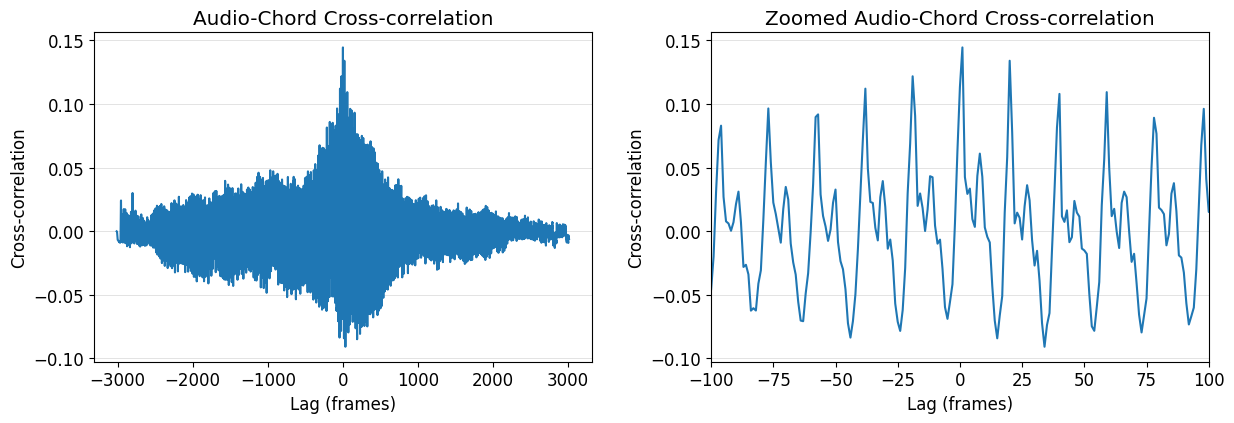
\includegraphics[width=1.0\textwidth]{figures/cross_correlation.png}
    \caption{Cross-correlation of the derivative of the CQT of the audio and the chord annotations for a single song. We can see correlation peaking in regular intervals of around 20 frames, which corresponds to one bar length in this song. On a larger scale, it is highest on around 0.}\label{fig:cross-correlation}
\end{figure}

To check alignment across the dataset, we can plot the lag of the maximum cross-correlations as a histogram. If we further assume that the annotations are not incorrect by more than approximately 10 seconds, this would mean we could restrict our maximum correlation search to a window of 100 frames either side of 0.  A histogram of maximum-lags per song is shown in Figure~\ref{fig:durations-and-lags} where the maximum is within a window of 100. This reduction does not change the shape of the picture. Rather, focusing on a reduced set of frames allows more detail to be visible. A final simple check was done by looking at the lengths of the audio and chord annotations. A histogram of differences in length is also shown in Figure~\ref{fig:durations-and-lags}. The majority of songs have a maximum lag in the region of 0, with a few outliers. This can be attrubted to noise. Furthermore, the majority of songs have a difference in length of 0, with a few outliers, almost all less than a second. This evidence combined with the qualitative analysis was convincing enough to leave the annotations as they are for training.

\begin{figure}[h]
    \centering
    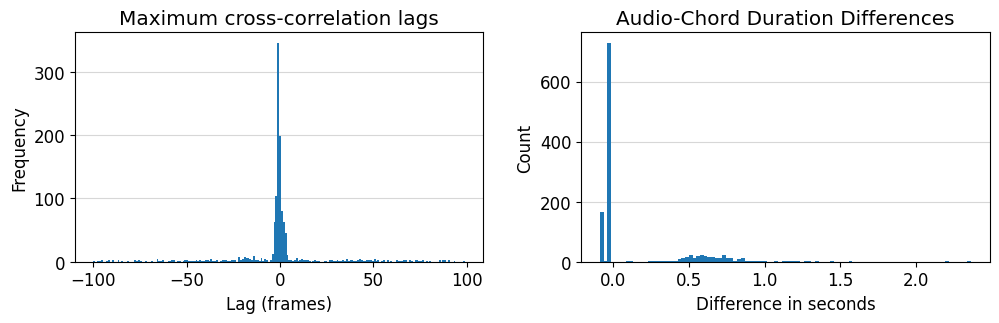
\includegraphics[width=1.0\textwidth]{figures/duration_diffs_and_lags.png}
    \caption{Cross-correlation of the derivative of the CQT of the audio and the chord annotations for a single song. The x-axis is the lag in frames and the y-axis is the correlation. The plot repeats every 100 frames, which corresponds to 4 bars.}\label{fig:durations-and-lags}
\end{figure}

\textbf{Incorrect and Subjective Annotations:} Throughout manual listening, no obviously wrong annotations were found. However, looking at songs which the first trained models perform the worst on, `Lovely Rita' by the Beatles sticks out. The model consistently guessed chords one semitone off, as if it thought the song was in a different key. Upon listening, it became clear that recording's tuning was not in standard A440 and so the song was removed. No other songs were found to have such issues.

Chord annotations are inherently subjective to some extent. Detailed examples in this dataset are given by~\citet{FourTimelyInsights}. They also note that there are several songs in the dataset of questionable relevance to ACR, as the music itself is not well-explained by chord annotations. However, these are kept in for consistency with other works as this dataset is often used in the literature. Some works decide to use the median as opposed to the mean accuracy in their evaluations in order to counteract the effect of such songs on performance~\citep{StructuredTraining}.

\subsubsection{Chord Distribution}

Much of the recent literature has focused on the long tail of the chord distribution~\citep{BalanceRandomForestACR,CurriculumLearning}, using a variety of methods to attempt to address the issue. It is first helpful to understand the distrbution of chords in the datasets, shown in Figure~\ref{fig:chord-distribution}. The distribution is broken down both by root and by quality, only for the larger chord vocabualary as the smaller vocabualary does not have the same long-tailed distribution. The plots clearly show that the distribution over qualities is highly skewed, with major and minor chords making up the majority of the dataset, and qualities like majorminor and diminished 7th chords having two to three orders of maginute fewer frames. Another helpful display of chord qualities can be found in the work by~\citet{ACRLargeVocab1}. The distribution over roots is far less skewed, although there is unsurprisingly a preference for chords from simpler keys like C, D or E and fewer in C\# or F\#.


\begin{figure}[h]
    \centering
    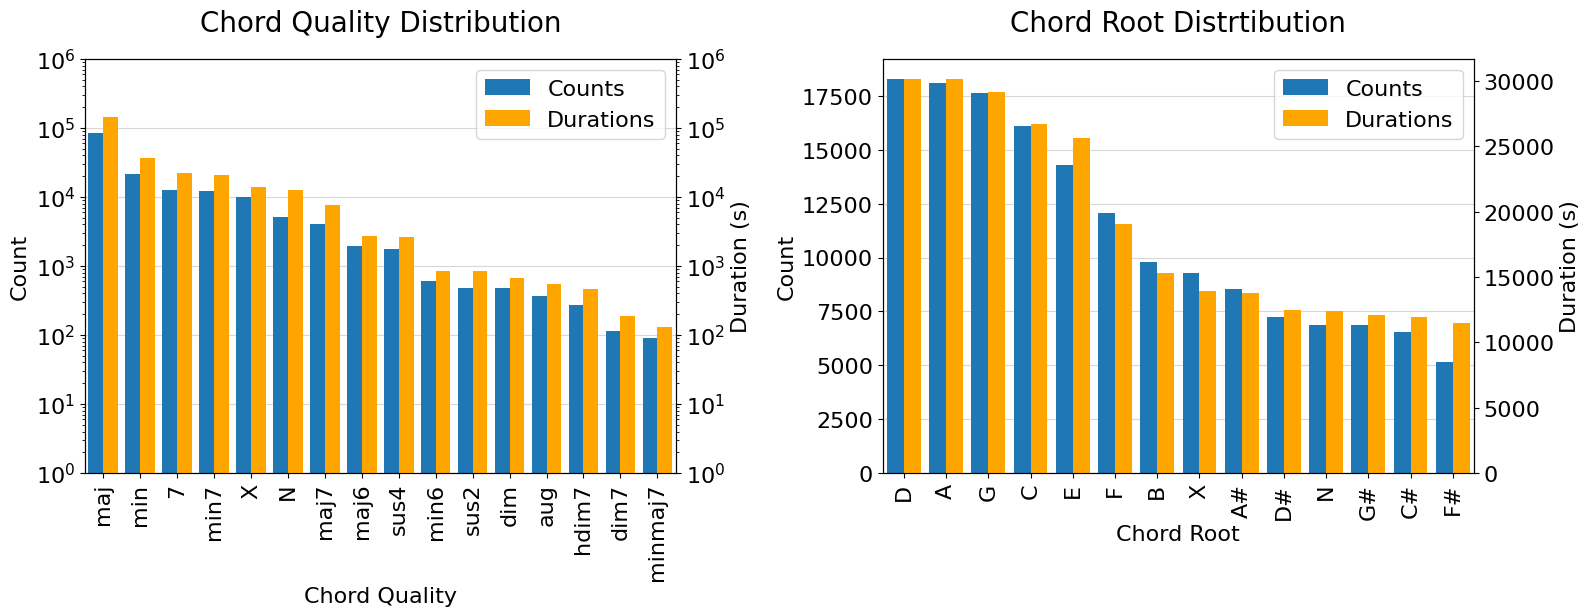
\includegraphics[width=1.0\textwidth]{figures/chord_distribution.png}
    \caption{Chord distributions in the \emph{Pop} dataset. The plots show both the raw counts in terms of frames and the duration in seconds for each chord root/quality. Note that the scales on the qualities are in log-scale. We observe that the qualities are very imbalanced, with \texttt{maj} the most popular, but that roots are relatively balanced.}\label{fig:chord-distribution}
\end{figure}


\subsection{JAAH Dataset}
I was warned by Andrea that the JAAH dataset has not been as commonly used as dataset the Billboard dataset. Therefore he could not guarantee that the audio was aligned for this dataset.

- As yet, JAAH is unused in this work
- Data was received as \texttt{.flac} files which were first converted to \texttt{.mp3} files to be in line with the Billboard dataset
- Comparison of the two datasets
- Description of the JAAH dataset and its use in this work
- Intended to be used as a test set to test the synthetic data generation.

\section{Evaluation}

We evaulated models using the standard \texttt{mir\_eval} library~\citep{mir_eval}. This library provides a variety of metrics for evaluating the performance of chord recognition models. The metrics used in this work follow standard practice, in using \texttt{root}, \texttt{third}, \texttt{seventh} and \texttt{mirex} accuracies. For a given hypothesis and reference chord, these metrics each return 1 if the root/third/seventh/three notes of the chord match and 0 otherwise. They return -1 if the true label is \texttt{X} and as such are ignored during evaluation. Finally, we looked at the overall frame-wise accuracy, called \texttt{frame}. We choose not to use \texttt{majmin}, \texttt{triad} or \texttt{tetrad} as these are highly correlated with the previous metrics. This makes sense from a theoretical standpoint as the third and seventh are strong indicators of the triad and tetrad of the chord. This was also verified empirically on some initial results, where the \texttt{third} and \texttt{majmin} accuraciest were always within 1\% of one another.

For the above metrics, the mean is computed for each song, and both the mean and median across songs are returned. Although, the mean and median were found to not be very different, the median was consistently slightly higher, likely due to there being more negative outliers than positive outliers. Some of these outliers could be those songs previously identified as being unsuitable for chordal analysis~\citep{FourTimelyInsights}. Because of the similarity between the two, we report only the mean throughout this work, chosen as it is more commonly used in recent literature. These metrics can be formally defined as follows:

\[ M(f) = \frac{1}{N} \sum_{i=1}^{N} \frac{1}{|\{t\in T : y_{i,t} \neq \texttt{X}\}|} \sum_{t\in T : y_{i,t} \neq \texttt{X}} f(y_{i,t}, \hat{y}_{i,t})\]

where $M$ is the metric in question, $f$ is a function which calculates the metric for a pair of reference and hypothesis chord labels, defined for each metric as above. $N$ is the number of songs, $T$ is the number of frames in a song, $y_{i,t}$ is the true chord at frame $t$ of song $i$, and $\hat{y}_{i,t}$ is the predicted chord at frame $t$ of song $i$.

For some experiments, we looked at three more metrics. The first is the overall frame-wise accuracy, calculated across the entire evaluation dataset rather than on a per-song basis, still ignoring \texttt{X} chords, called \texttt{frame}\textsubscript{all}. The second and third are the mean and median class-wise accuracies, called \texttt{class}\textsubscript{mean} and \texttt{class}\textsubscript{median} respectively. These are the mean/median accuracy over each chord class. These metrics are formally defined as follows:

\[\text{frame}\textsubscript{all} = \frac{1}{N} \sum_{i=1}^{N} \frac{1}{|\{t\in T : y_{i,t} \neq \texttt{X}\}|} \sum_{t\in T : y_{i,t} \neq \texttt{X}} \mathbbm{1}_{(y_{i,t} = \hat{y}_{i,t})}\]
\[
\text{class}\textsubscript{mean} = \frac{1}{C} \sum_{c=1}^{C} \text{acc}(c), \quad
\text{class}\textsubscript{median} = \text{median}_{c=1}^{C} [\text{acc}(c)]
\]

where $\text{acc}(c)$ is the accuracy of class $c$ defined as:

\[\text{acc}(c) = \frac{\sum_{i=1}^{N} \sum_{t\in T : y_{i,t} \neq \texttt{X}} \mathbbm{1}_{(y_{i,t} = c \land \hat{y}_{i,t} = c)}}{\sum_{i=1}^{N} \sum_{t\in T : y_{i,t} \neq \texttt{X}} \mathbbm{1}_{(y_{i,t} = c)}}\]


where $C$ is the number of chord classes, and $N$, $T$, $y_{i,t}$ and $\hat{y}_{i,t}$ are as defined before.

This metric is intended to measure the model's performance on the long tail of the chord distribution. It is important to measure both the mean and median as the distribution of accuracies is skewed. These last two metrics are the only ones take into account the entire evaluation dataset at once. Some songs may contain very few chords of a particular chord or quality, making the per-song metrics very noisy.

For the majority of experiments, the metrics on the validation set are used to compare performance. The test set is held out for use only to compare the final performances of selected models.

Finally, other evaluation tools were used, such as confusion matrices and accuracies over particular chord qualities and classes. A small amount of qualitative analysis was also done, looking at the predictions of the model on a few songs. This was done to understand the model's behaviour and to identify any systematic errors.

\section{Training}

Three variants of the dataset were used for training, validation and testing. For training, an epoch consisted of randomly sampling a patch of audio from each song in the training set. The length of this sample was kept as a hyperparameter, set to 28 seconds for the majority of experiments. For testing, the entire song was used was performance was found to be better if the model was allowed to see the entire song at once. Because songs are of variable length, songs were split into patches of the same length as the training patches when validating mid-way through training. This meant that computation could be parallelised without many padded frames. For all variants, frames in the batch were padded to the maximum length of the batch and ignored for loss or metric calculation.

The models were trained using the \texttt{PyTorch} library~\citep{pytorch}. All final experiments were run on the ML Teaching Cluster with a variety of Nvidia GPUs, mostly GTX 1060's or GTX 1080's. Unless state otherwise, models were trained with the Adam optimiser~\citep{adam} with a learning rate of $0.001$ and pytorch's \texttt{CosineAnnealingLR} scheduler, set to reduce the learning rate to 1/10th of its initial value over the run. Models were trained to minimise the cross entropy loss between the predicted chord and the true chord distributions. The models were trained with a batch size of 64 for a maximum of 150 epochs unless stated otherwise. This batch size was based on brief experiments testing the speed of an epoch. Validation was conducted every 5 epochs in order to save on computation time. Optionally, training was stopped early if the validation loss did not improve for 25 epochs. The model was saved whenever the validation loss improved. Each training run took approximately 30 minutes of GPU time. 

For the majority of experiments, a random 60/20/20\% training/validation/test split was used. This contrasts much of the literature which uses a 5-fold cross validation split, as introduced by~\citet{FourTimelyInsights}. We do not maintain this split in order to obtain clean estimators of the generalisation error using the held-out test set. The split was kept constant across experiments. Later, models were re-trained on the combined training and validation sets and tested on the test set. In Chapter~\ref{chap:synthetic_data}, the models were trained on the entire \emph{Pop} dataset and tested on the \emph{JAAH} dataset.